\documentclass{beamer} 
\usepackage{beamerthemeTUM}
\usepackage[latin1]{inputenc} 
\usepackage{amsmath} 
\usepackage{amsfonts} 
\usepackage{amssymb} 
\usepackage{algorithm} 
\usepackage{algorithmic} 
\usepackage{multicol} 
\usepackage{url}
\usepackage{graphics}
\usepackage{multicol}
\usepackage{eso-pic}
%\usepackage{pst-node}
\usepackage{xcolor}
\usepackage{multido}
\usepackage{subfigure}
%\usepackage{pstricks}
%\usepackage{pstricks-add}
%\usepackage{pst-grad}
%\usepackage{float} 

\graphicspath{{figures/}}

\setlang{en}


\author{Sebastian Lehnerer} 
\title{Multilabel Attribute Selection} 

\subtitle{Tanimoto Distance}
\email{lehnerer@in.tum.de}
\date{\today}
\institute[2011]{Technische Universit\"at M\"unchen}


\begin{document} 


\AddToShipoutPicture{\TitlePicture}
\maketitle
%\frame{\titlepage}
\ClearShipoutPicture
\AddToShipoutPicture{\BackgroundPicture}
\AtBeginPart{\frame{\partpage}}

\frame{
 {\insertsection} 
 \begin{itemize} 
  \item feature selection for every label, where other labels are
    treated as normal features
    \end{itemize} 
    \begin{eqnarray*} 
      Y_{1} &\leftarrow & \{X_{1}...X_{n} \cup Y_{2}...Y_{n}|X_{i},Y_{i}\in\{0,1\}\}\\ 
      Y_{2} &\leftarrow & \{X_{1}...X_{n} \cup Y_{1},Y_{3}...Y_{n}|X_{i},Y_{i}\in\{0,1\}\}\\ 
      &\vdots &\\ 
      Y_{n} &\leftarrow & \{X_{1}...X_{n} \cup Y_{1}...Y_{n-1}|X_{i},Y_{i}\in\{0,1\}\} 
    \end{eqnarray*} 
  
}

\frame{
 {\insertsection} 
  \begin{itemize}
  	\item using label feature sets as vectors $ <0,1,0,0,1,0,\cdots,1,0> $      
  	\item Hierachical Clustering using the Tanimoto Distance.
  	\begin{equation*}
		T_s(X,Y) =  \frac{\sum_i ( X_i \land Y_i)}{\sum_i ( X_i \lor Y_i)}
	\end{equation*}
  	\item Single, Complete, Average and Mean Clustering
  	\item no. of clusters: $2,4,6$
  \end{itemize} 
}

\frame{
 {\insertsection} 
		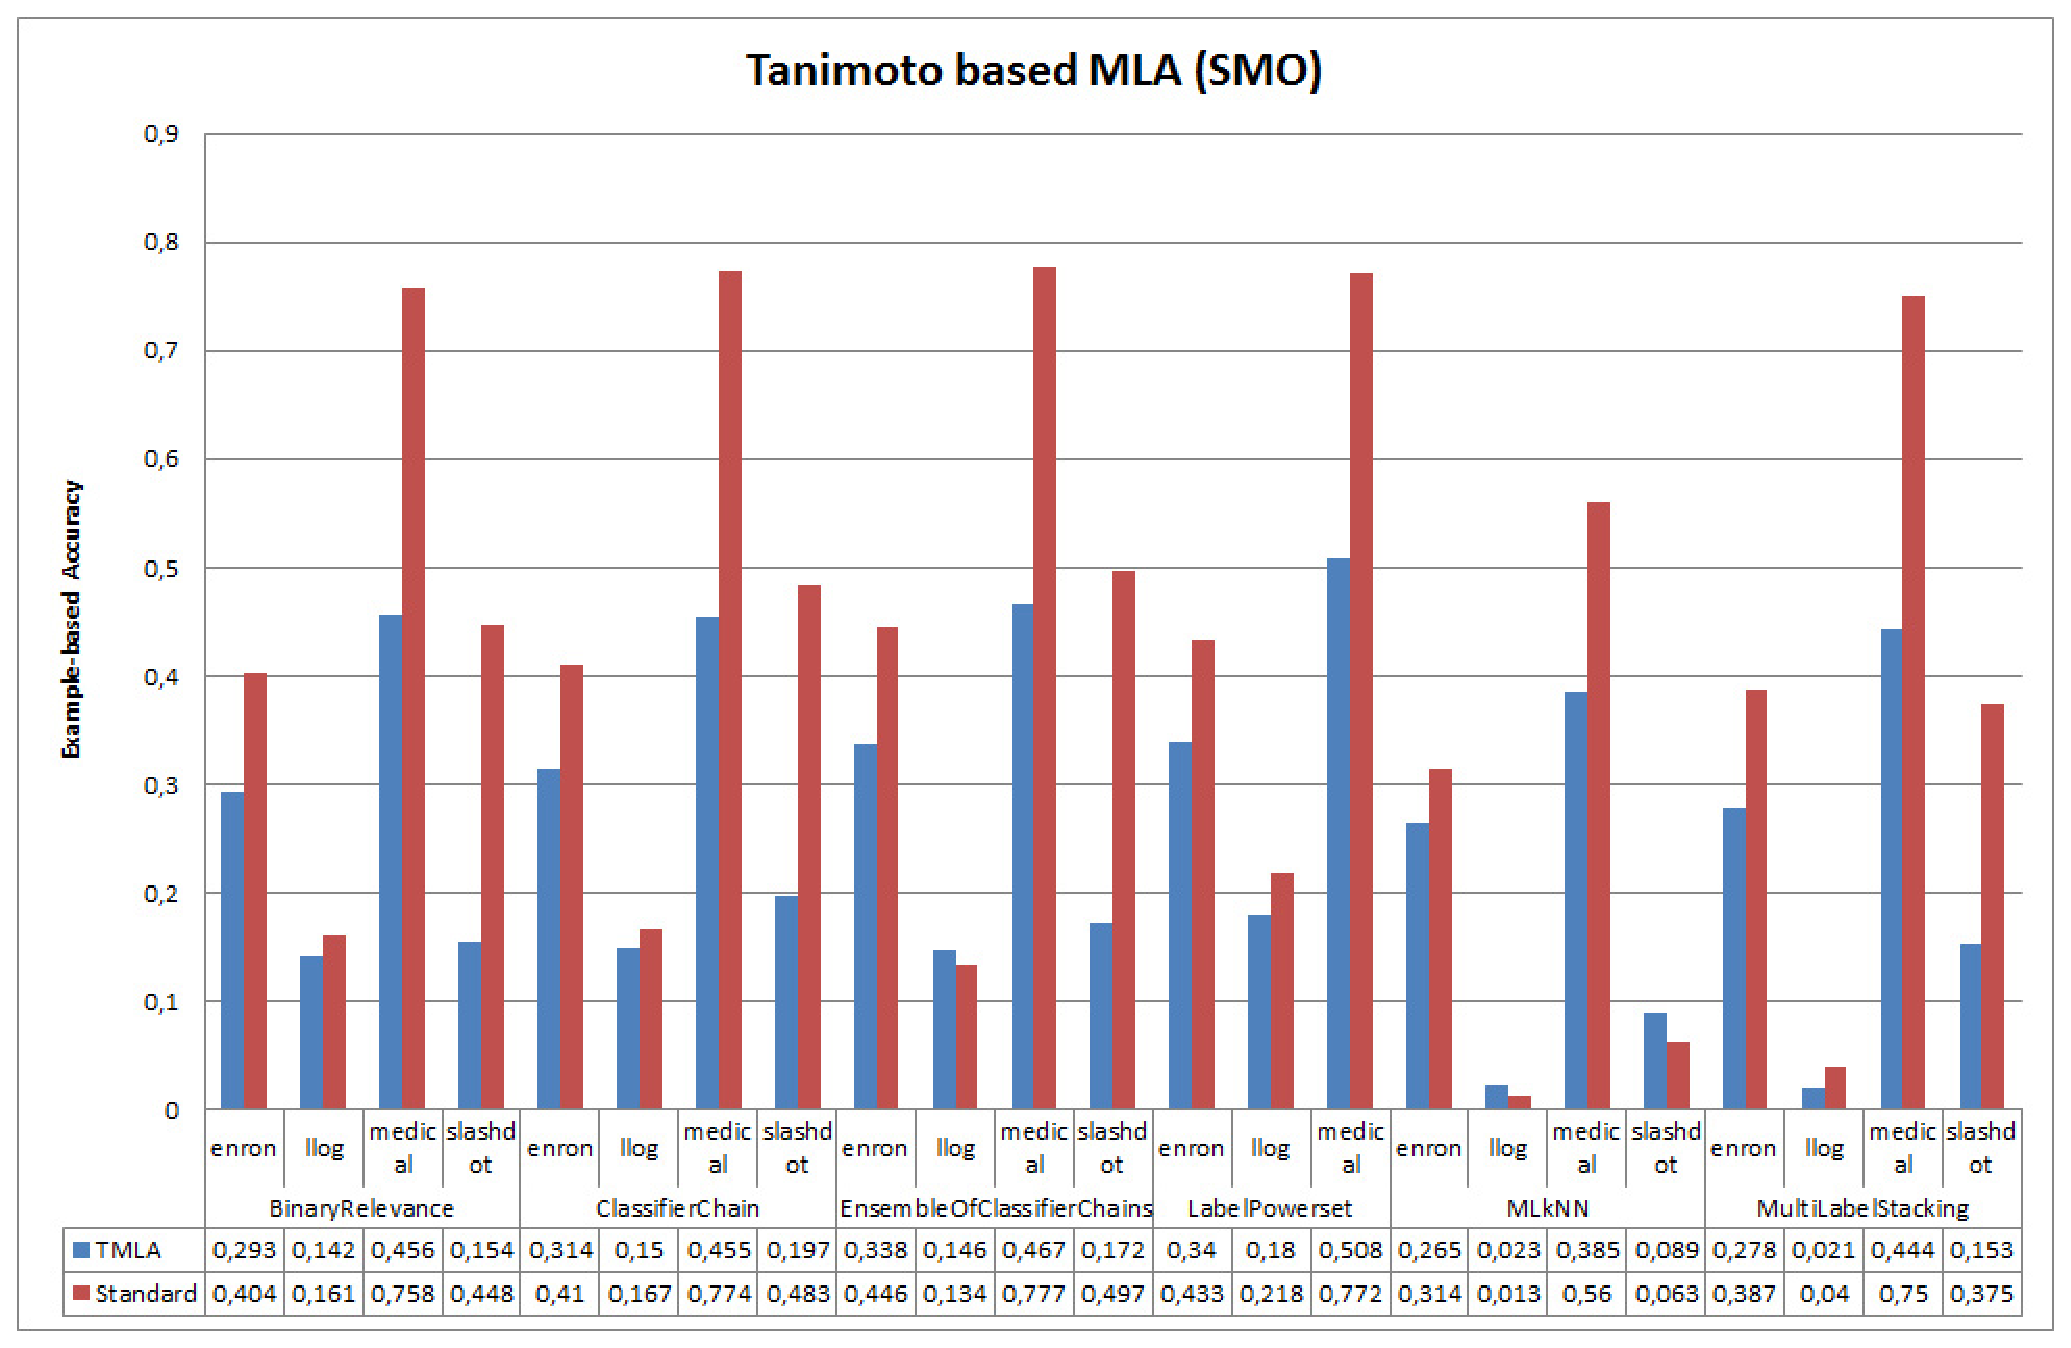
\includegraphics[scale=.3]{figures/tmla_results_smo.eps}
}

\frame{
 {\insertsection} 
		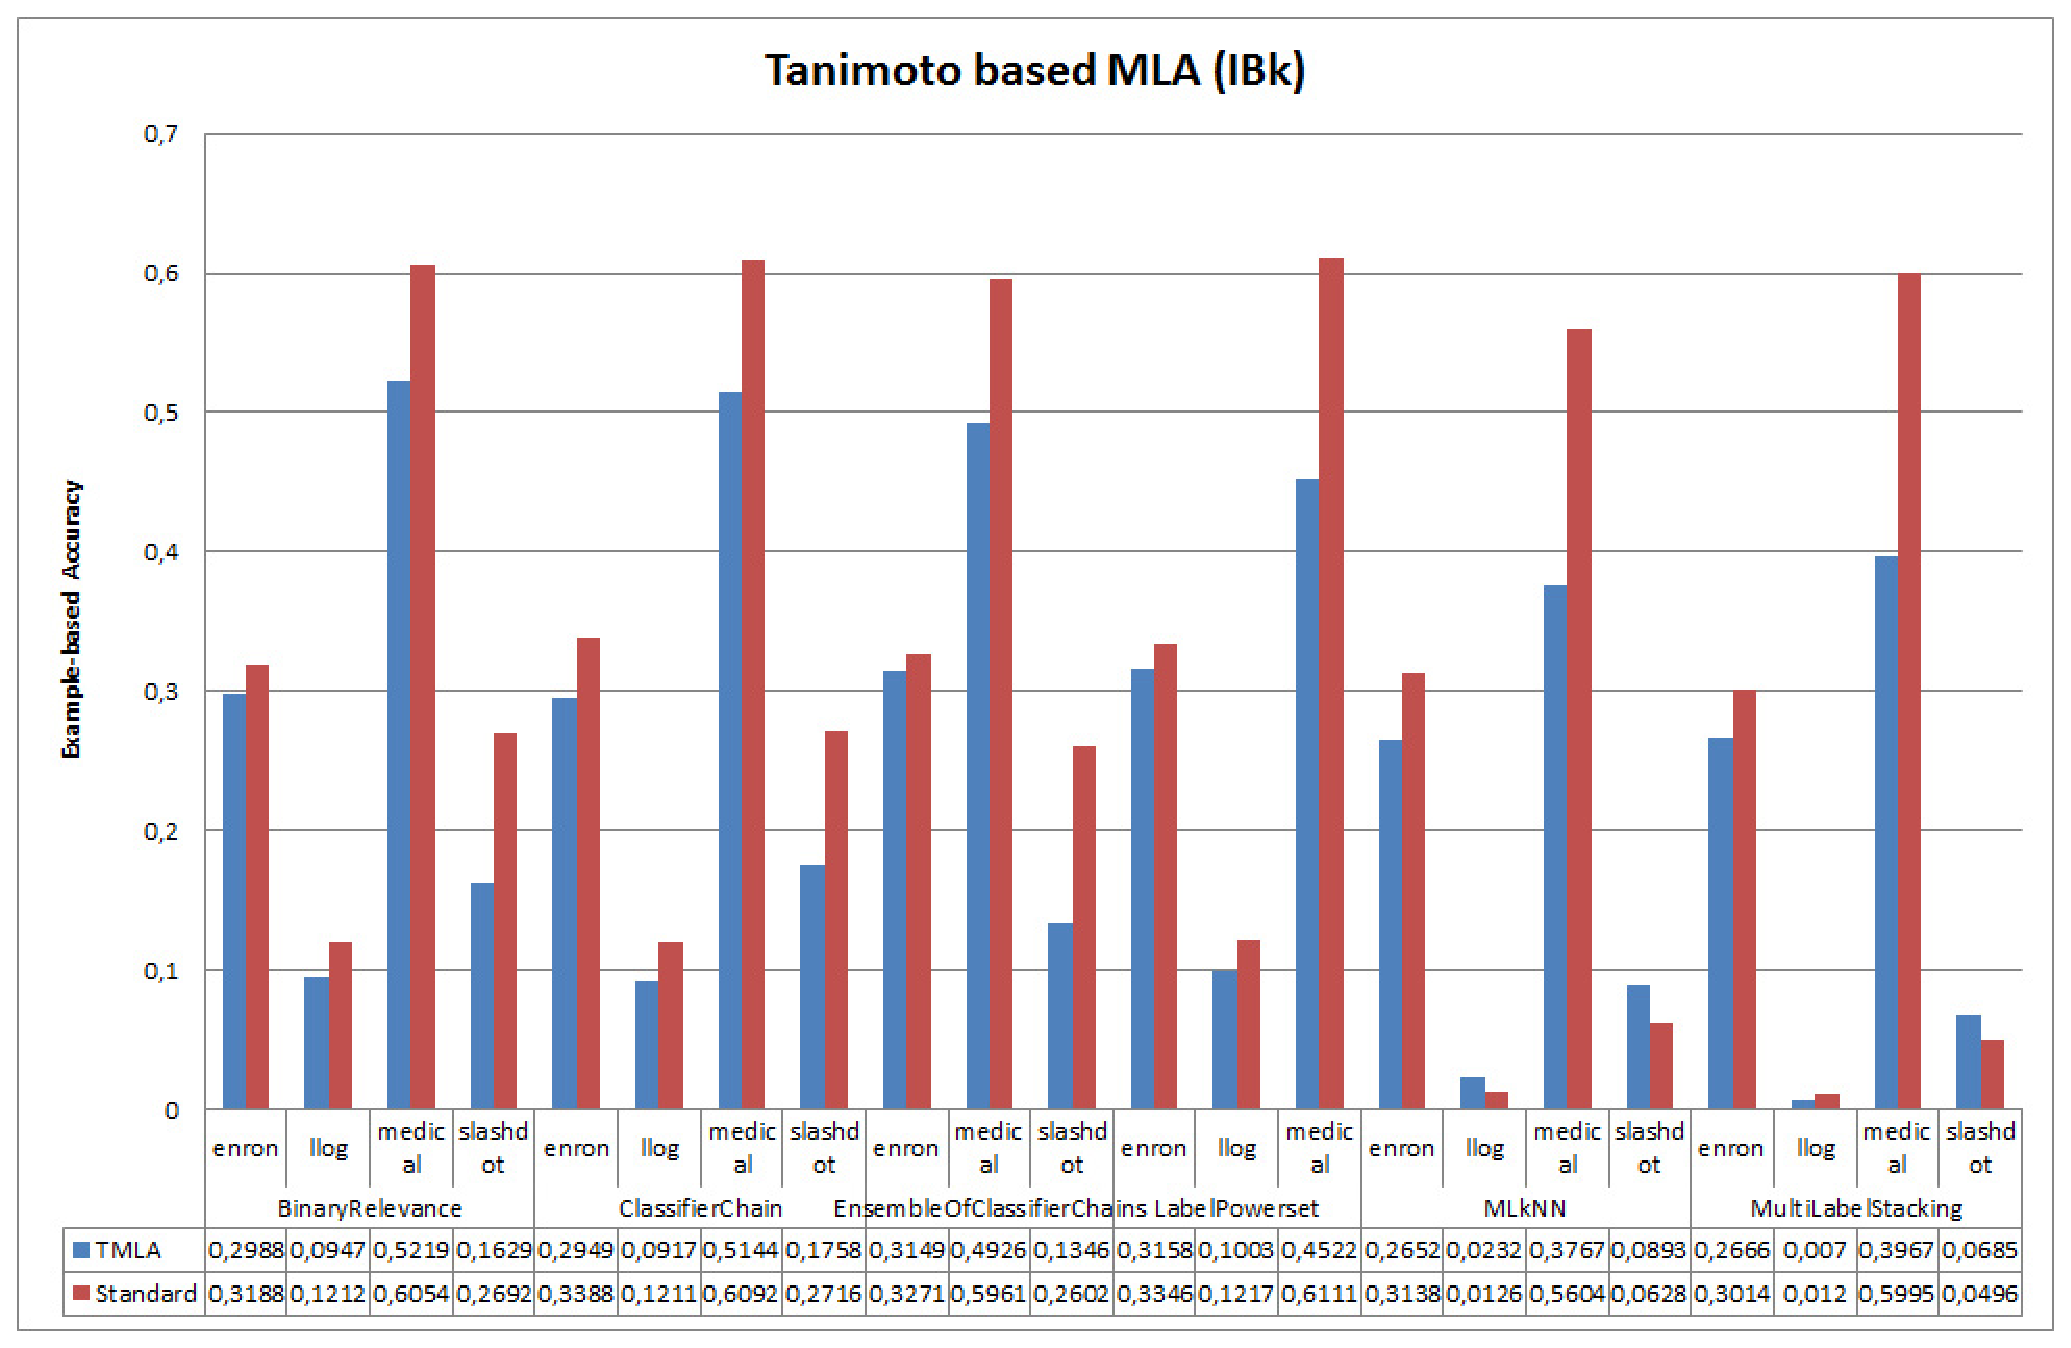
\includegraphics[scale=.3]{figures/tmla_results_ibk.eps}
}

\frame{
 {\insertsection} 
		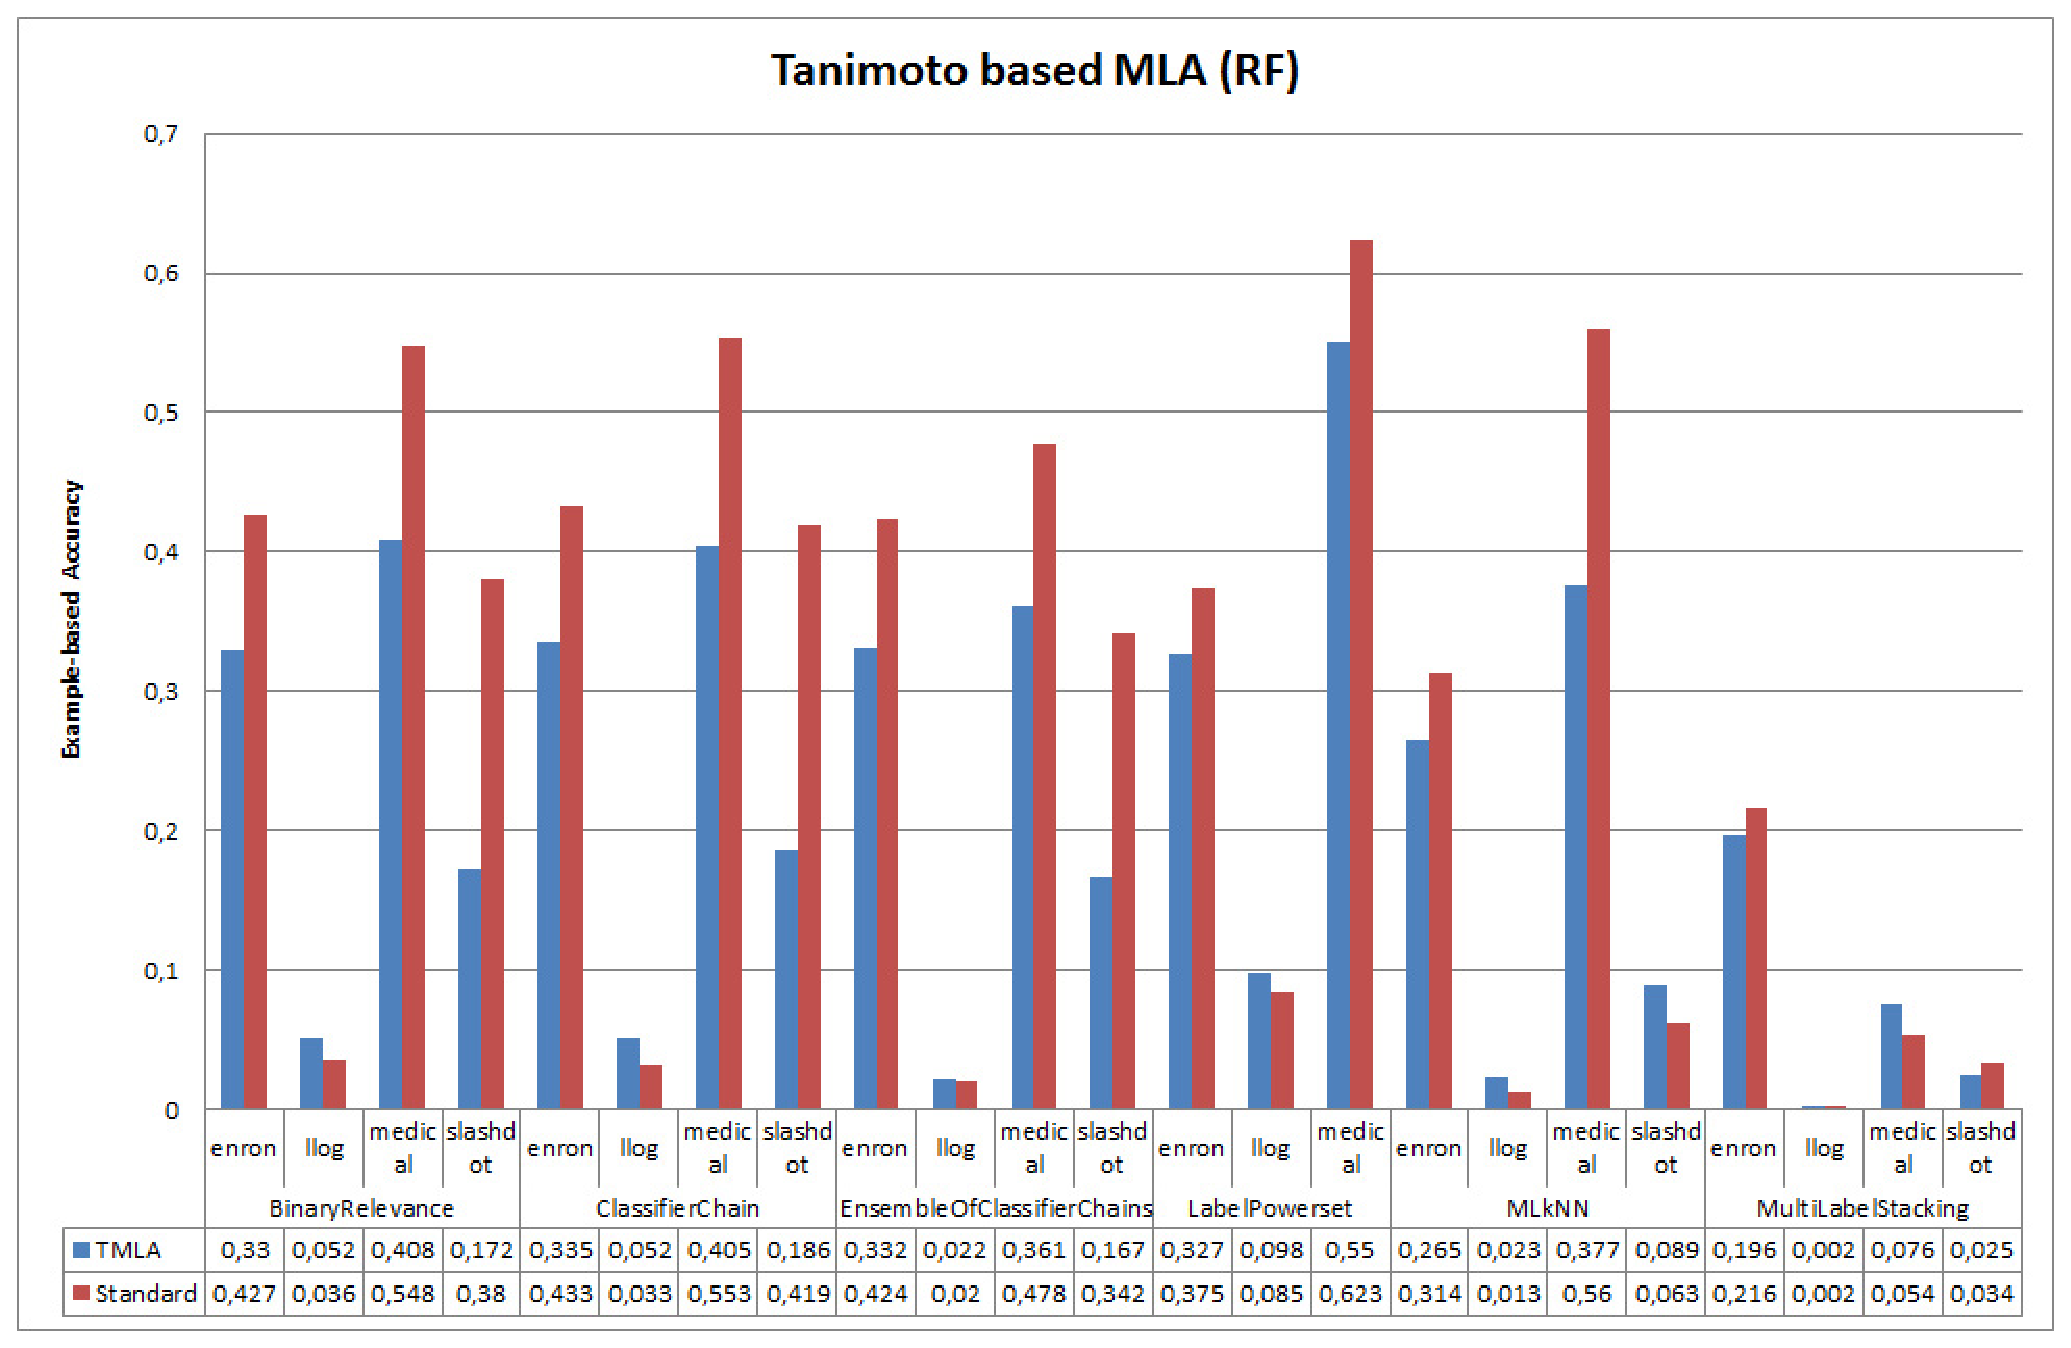
\includegraphics[scale=.3]{figures/tmla_results_rf.eps} 
}

\frame{
	{\insertsection}
	example cluster characteristics (\(\varnothing\) over folds)
	\scriptsize {s
	\begin{itemize}
	  	\item enron\\
		\(\varnothing\) number of clusters : 2\\
		\(\varnothing\) number of clusters ($> 2$ labels) : 2\\
		\(\varnothing\) number of labels per cluster: 31
		\item llog\\
		\(\varnothing\) number of clusters : 2\\
		\(\varnothing\) number of cluster ($> 2$ labels) : 1.8\\
		\(\varnothing\) number of labels per cluster: 40,60	
		\item medical\\
		\(\varnothing\) number of clusters : 6\\
		\(\varnothing\) number of cluster ($> 2$ labels) : 2\\
		\(\varnothing\) number of labels per cluster: 8,9	
		\item slashdot\\
		\(\varnothing\) number of clusters : 2\\
		\(\varnothing\) number of cluster ($> 2$ labels) : 1.8\\
		\(\varnothing\) number of labels per cluster: 14.90	
	\end{itemize}
}
}

\end{document}